\documentclass{article}%
\usepackage[T1]{fontenc}%
\usepackage[utf8]{inputenc}%
\usepackage{lmodern}%
\usepackage{textcomp}%
\usepackage{lastpage}%
\usepackage[head=40pt,margin=0.5in,bottom=0.6in]{geometry}%
\usepackage{graphicx}%
%
\title{\textbf{De Grazia: Esta amenaza me genera zozobra por lo que me pueda ocurrir}}%
\author{Giselle Goncalves | @GiselleAGP}%
\date{14/11/2018}%
%
\begin{document}%
\normalsize%
\maketitle%
\textbf{URL: }%
http://www.el{-}nacional.com/noticias/oposicion/grazia{-}esta{-}amenaza{-}genera{-}zozobra{-}por{-}que{-}pueda{-}ocurrir\_259810\newline%
%
\textbf{Periodico: }%
EN, %
ID: %
259810, %
Seccion: %
Oposición\newline%
%
\textbf{Palabras Claves: }%
Diputados, Política, Asamblea Nacional, Bolívar\newline%
%
\textbf{Derecho: }%
1.3%
, Otros Derechos: %
17%
, Sub Derechos: %
1.3.4%
\newline%
%
\textbf{EP: }%
NO\newline%
\newline%
%
\textbf{\textit{El diputado a la Asamblea Nacional explicó que el comisionado de la Dirección General de Contrainteligencia Militar planificaría asesinarlo a él y al dirigente Andrés Velázquez}}%
\newline%
\newline%
%
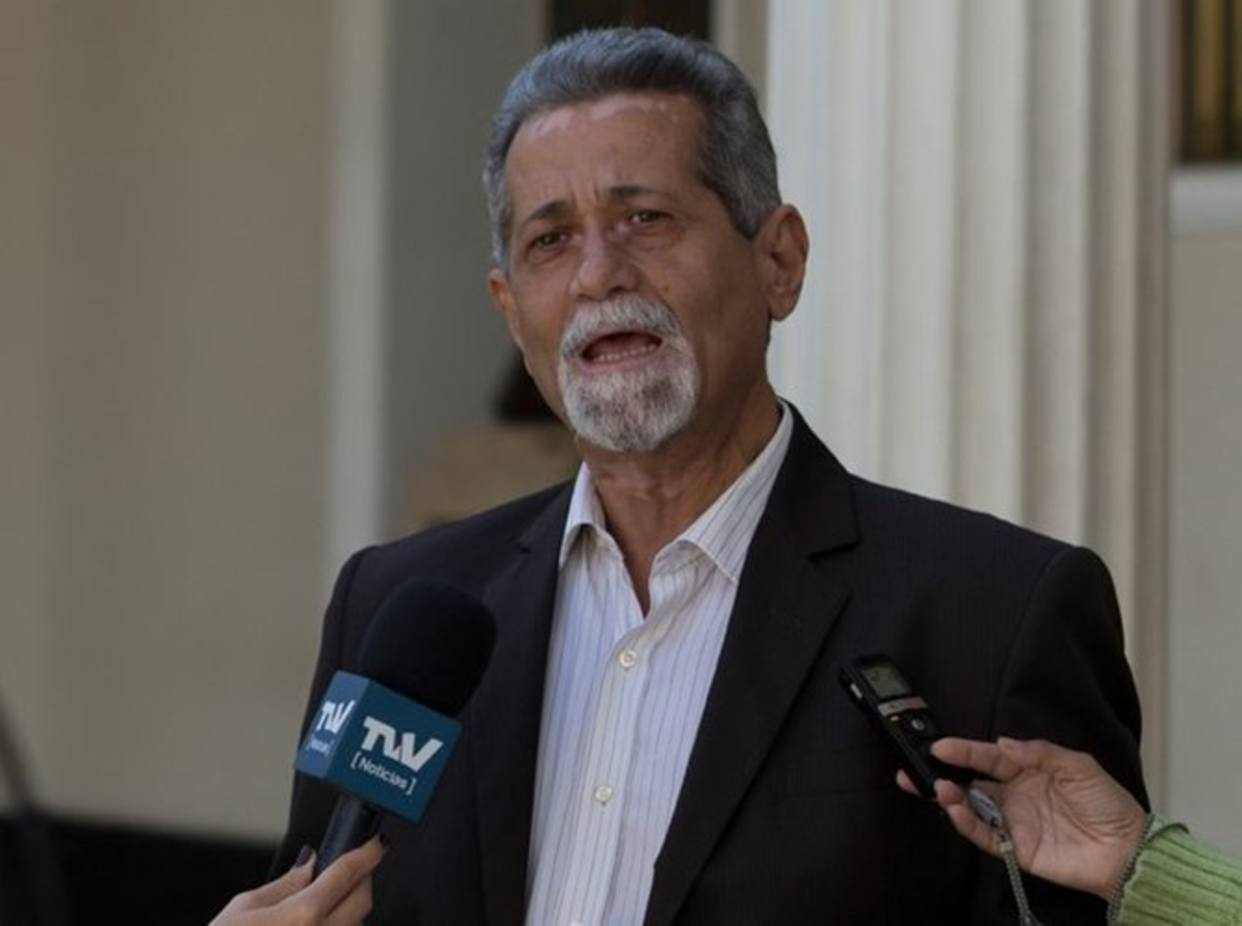
\includegraphics[width=300px]{168.jpg}%
\newline%
%
Américo De Grazia, diputado a la Asamblea Nacional, denunció este miércoles que un miembro de la Dirección General de Contrainteligencia Militar (Dgcim) fue designado para “neutralizar” al parlamentario y a Andrés Velázquez, dirigente político del estado Bolívar.%
\newline%
%
“La información nos llegó este martes, un Dgcim de nombre Alexander Gramcko Arteaga, quien es el segundo a bordo de esta organización en el estado Bolívar y tiene como propósito, según ellos, neutralizarnos”, explicó el diputado en una entrevista exclusiva a~El Nacional Web.%
\newline%
%
Aseguró que en términos policiales, neutralizar es el equivalente a desaparecer, extinguir o matar. Señaló que este agente del cuerpo de seguridad labora directamente en el estado Bolívar, y que la información fue atribuida por los integrantes de la Dgcim.%
\newline%
%
De Grazia indicó que este funcionario tiene antecedentes penales, incluso una denuncia hecha por Tamara Sujú, abogada especialista en derechos humanos, ante la Corte Penal Internacional. “Me lo vendieron como un chico malo”, aseguró el diputado.%
\newline%
%
Puntualizó que Gramcko no es un sujeto fácil identificable. Los amenazados recibieron fotos en las que muestran su rostro, pero al comprobarlas, se notó que no son verídicas.%
\newline%
%
“Al revisar en las redes sociales, aparece con un rostro y en otro lado aparece con otro. Y cuando lo tiene, ~a veces tiene barba, a veces está sin cabello, no sabemos si las cambian. Es alguien que se escabulle del ojo público”, detalló Américo.%
\newline%
%
Aunque no han recibido una acción directa con respecto a esta amenaza, se pudo conocer por Mariela Magallanes, diputada al Parlamento, que le han realizado seguimiento a la esposa de Velásquez y a la hija, esperando que ingrese y salga de su escuela. “Esto genera zozobra porque no sabemos exactamente qué es lo que puede ocurrir”.%
\newline%
%
En su última visita a Guayana, estado Bolívar, indicó que no pudo acercarse a su casa. “No pude ni visitar mi casa porque un carro que no tenía identificación de ningún tipo estuvo en mi residencia, lo que produce incertidumbre. Hemos hecho denuncias públicas pero no es suficiente”, aseveró el parlamentario.%
\newline%
%
Mientras mantengan las amenazas, los dirigentes políticos se mantendrán bajo perfil. ~“Hemos solicitado el apoyo internacional de las organismos y pronto levantaremos un informe que le hace seguimiento a la medida cautelar que me fue otorgada por~los hechos en Tumeremo”, discernió De Grazia.%
\newline%
%
“Todo el mundo sabe que nosotros no tenemos armas, no tenemos guardaespaldas, no tenemos choferes, escoltas ni como pagarlos como para responder ante enfrentamientos. Es una situación de desventaja muy grande y es por ello que preferimos recurrir a la opinión pública”, ratificó.%
\newline%
%
\end{document}